% \documentclass{article}
\documentclass[../../outputs/main.tex]{subfiles}

% Any packages or configurations specific to this section
\usepackage{lipsum}
\usepackage{graphicx}

\begin{document}

\subsubsection{Comparison between MPCOPF and MPDOPF}
In this section, comparative analyses are carried out between MPCOPF and MPDOPF considering 5-hour time steps.


\begin{table}[h!]
    \centering
    \caption{Comparative analyses between MPCOPF and MPDOPF}
    \begin{tabular}{|l|c|c|}
    \hline
    \textbf{Metric} & \textbf{MPCOPF} & \textbf{MPDOPF} \\ \hline
    Line loss (kW) &   &  \\ \hline
    Substation real power (kW) &    &   \\ \hline
    Substation reactive power (kVAR) &    &   \\ \hline
    PV real power (kW) &    &    \\ \hline
    PV reactive power (kVAR) &    &   \\ \hline
    Substation power cost (\$) &     &   \\ \hline
    \end{tabular}
    \label{table:combined_results_slim}
\end{table}


Further, here the 

\begin{table}[h!]
    \centering
    \caption{ACOPF feasibility analyses}
    \begin{tabular}{|l|c|c|c|}
    \hline
    \textbf{Metric} & \textbf{MPDOPF} & \textbf{OpenDSS} \\ \hline
    Line loss (kW) &   &  \\ \hline
    Substation real power (kW) &    &   \\ \hline
    Substation reactive power (kVAR) &    &   \\ \hline
    Max. voltage discrepancy (pu) &    &    \\ \hline
    Max. line loss discrepancy (pu) &    &   \\ \hline
    Max. substation power discrepancy (pu) &     &   \\ \hline
    \end{tabular}
    \label{table:feas-5-}
\end{table}


\textcolor{red}{Boundary Variable Plots are too tall, make them slightly shorter, like 25\% of the page only. Also their caption sizes are apparently wrong, so fix that.}

\begin{figure*}[h!]
    \centering
    % Row 1
    \begin{subfigure}[b]{0.3\textwidth}
        \centering
        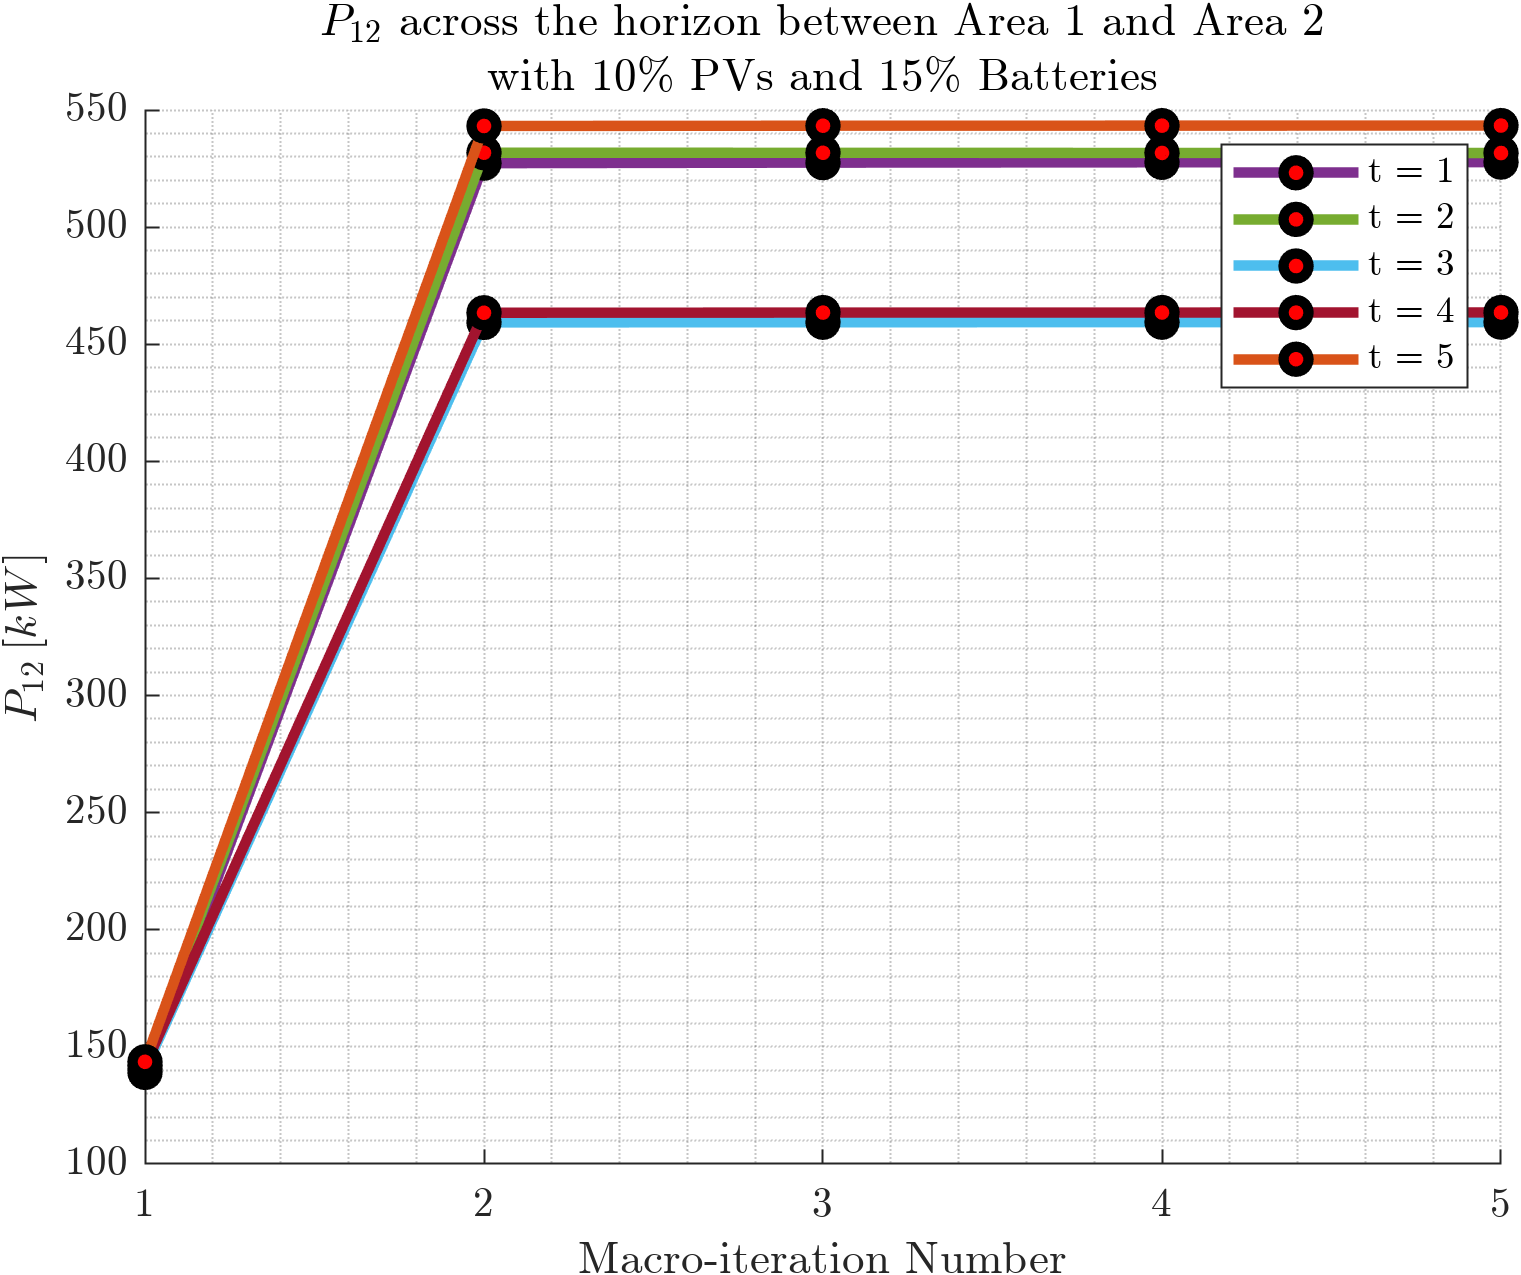
\includegraphics[width=\textwidth]{../figures/T5-pv10-batt15-PBoundary/BoundaryRealPower_vs_t_vs_macroItr_5Areas_1_2_genCost_pv_10_batt_15_.png}
        \caption{Real Power: Area 1 to Area 2}
        \label{fig:real_power_1_2}
    \end{subfigure}
    \hfill
    \begin{subfigure}[b]{0.3\textwidth}
        \centering
        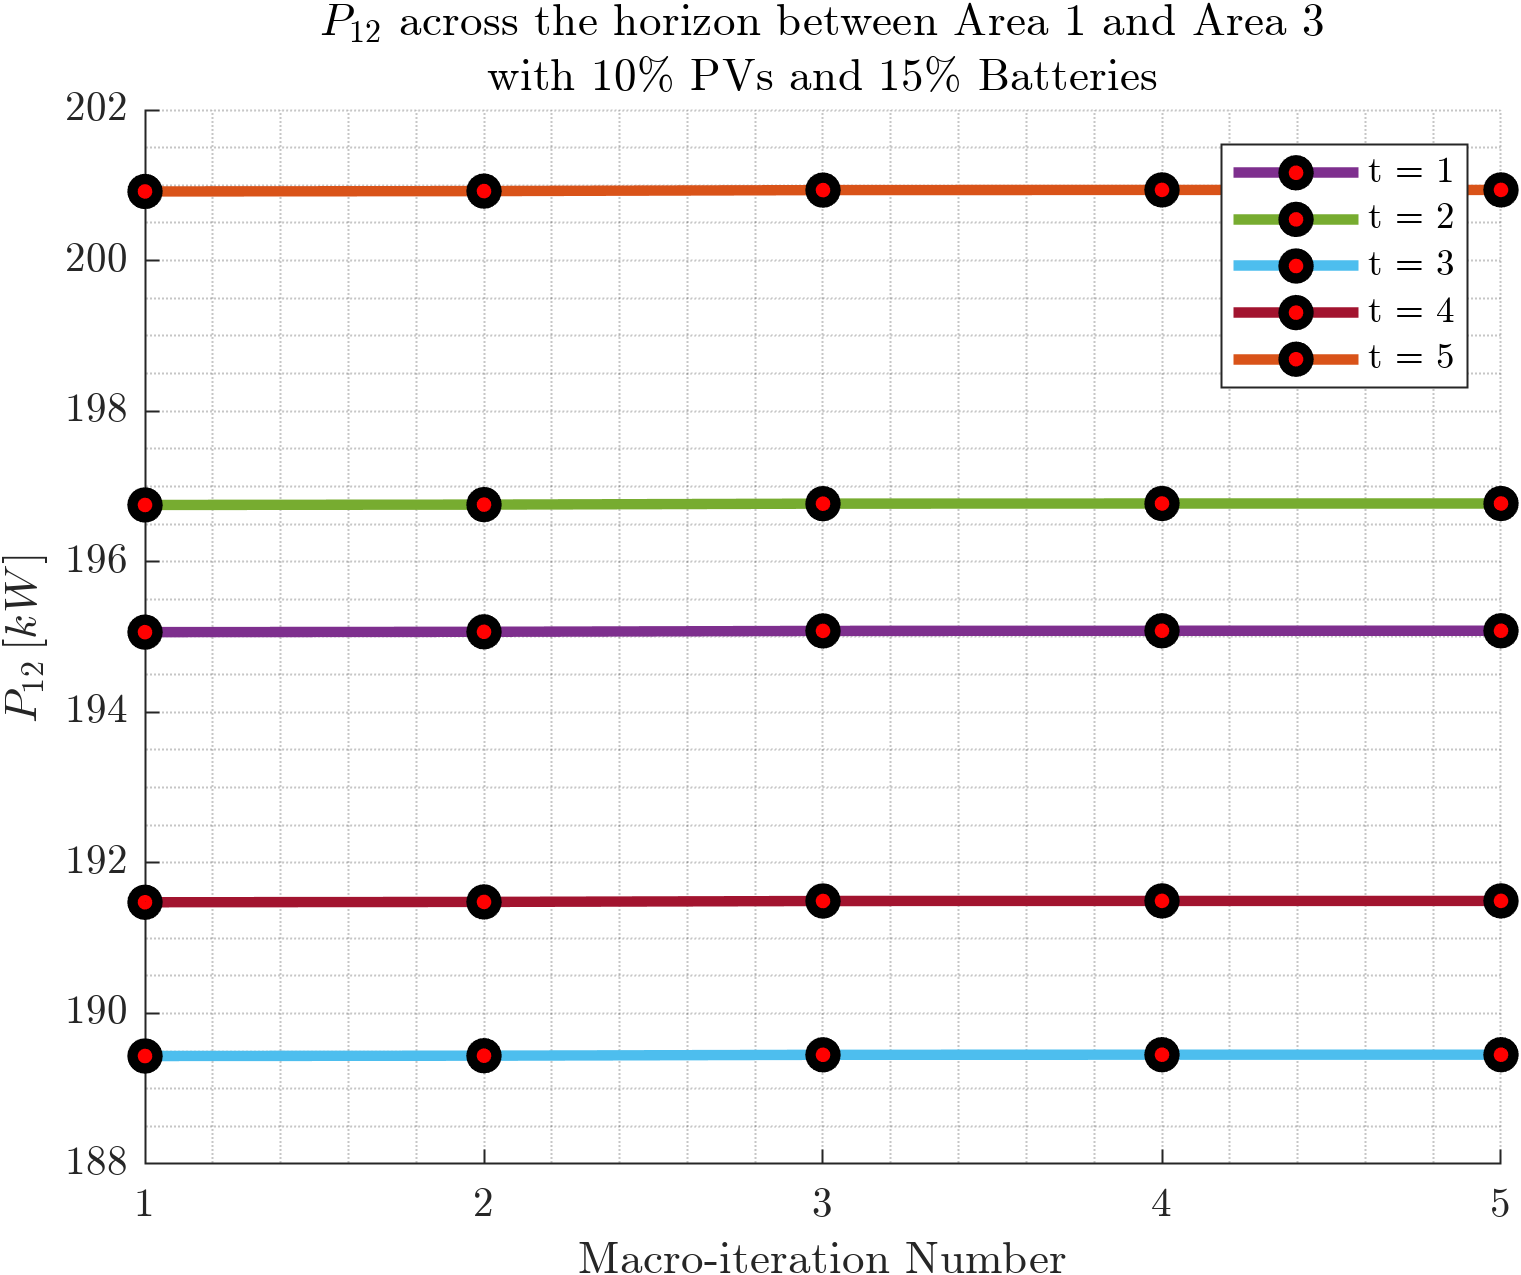
\includegraphics[width=\textwidth]{../figures/T5-pv10-batt15-PBoundary/BoundaryRealPower_vs_t_vs_macroItr_5Areas_1_3_genCost_pv_10_batt_15_.png}
        \caption{Real Power: Area 1 to Area 3}
        \label{fig:real_power_1_3}
    \end{subfigure}
    \hfill
    \begin{subfigure}[b]{0.3\textwidth}
        \centering
        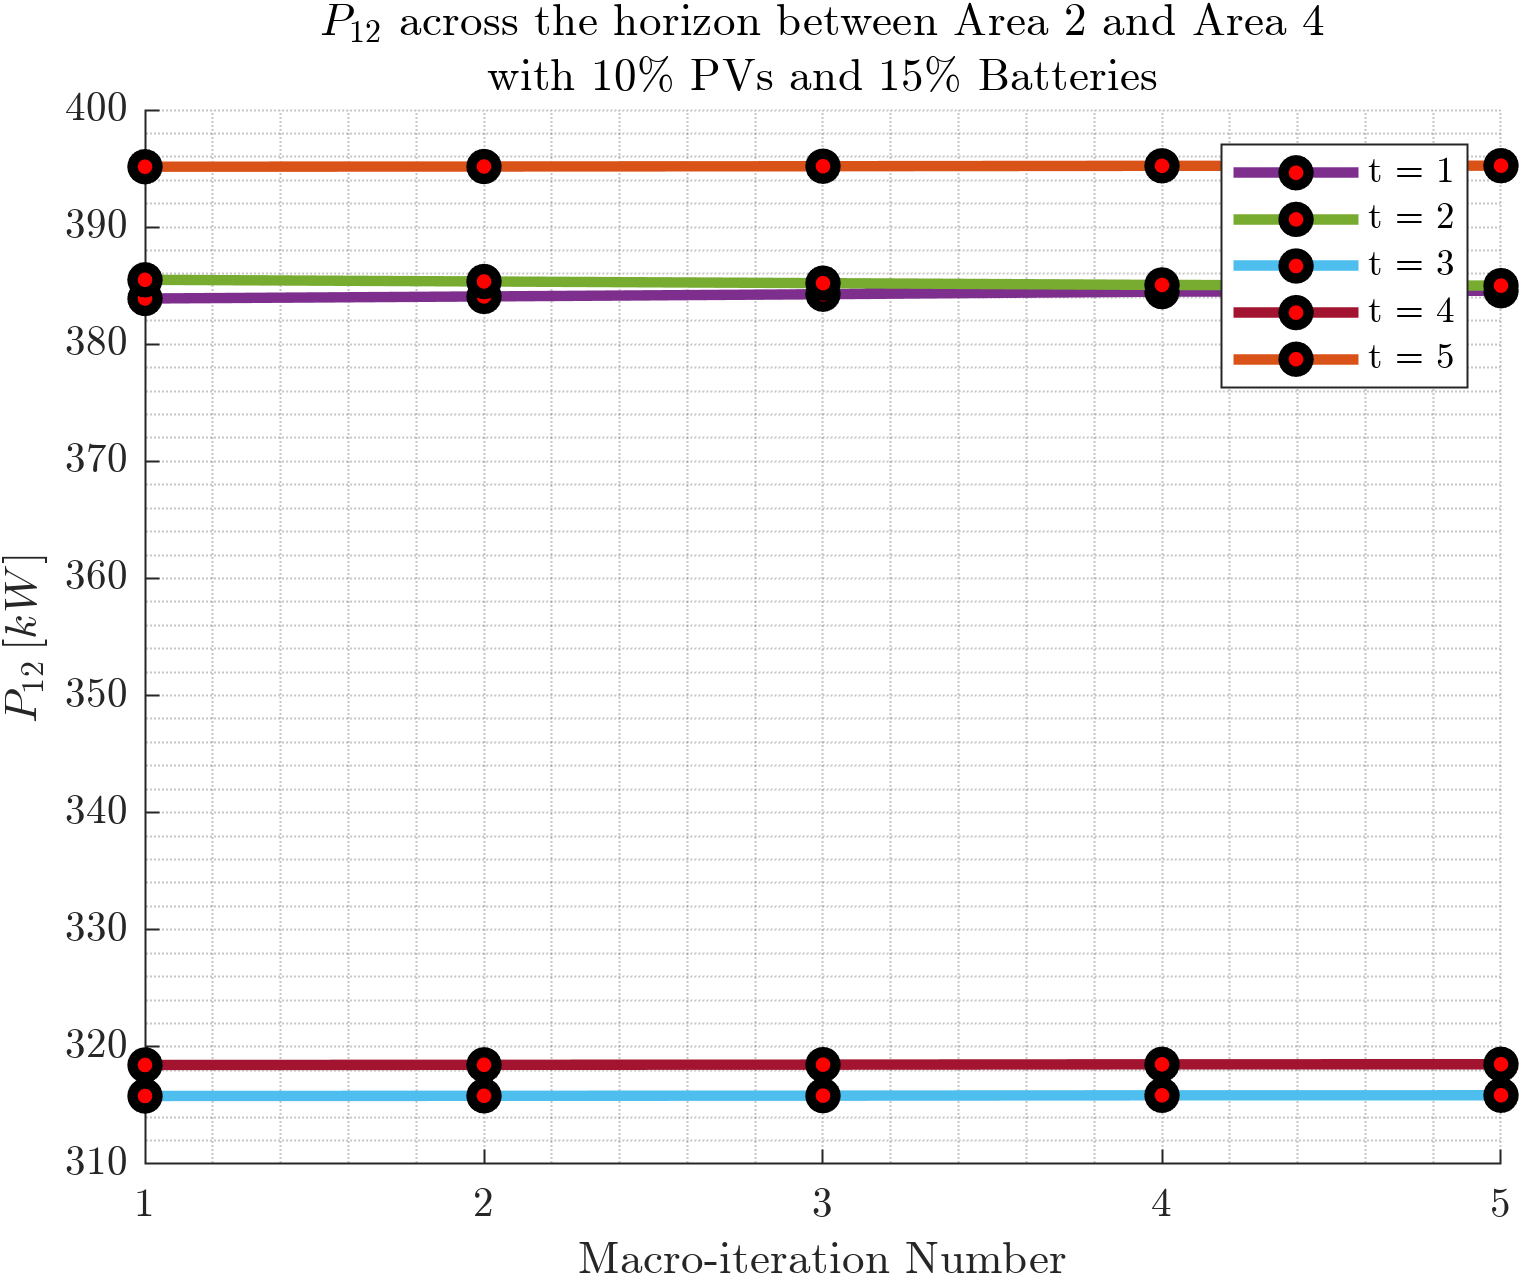
\includegraphics[width=\textwidth]{../figures/T5-pv10-batt15-PBoundary/BoundaryRealPower_vs_t_vs_macroItr_5Areas_2_4_genCost_pv_10_batt_15_.png}
        \caption{Real Power: Area 2 to Area 4}
        \label{fig:real_power_2_4}
    \end{subfigure}
    
    % Row 2
    \begin{subfigure}[b]{0.3\textwidth}
        \centering
        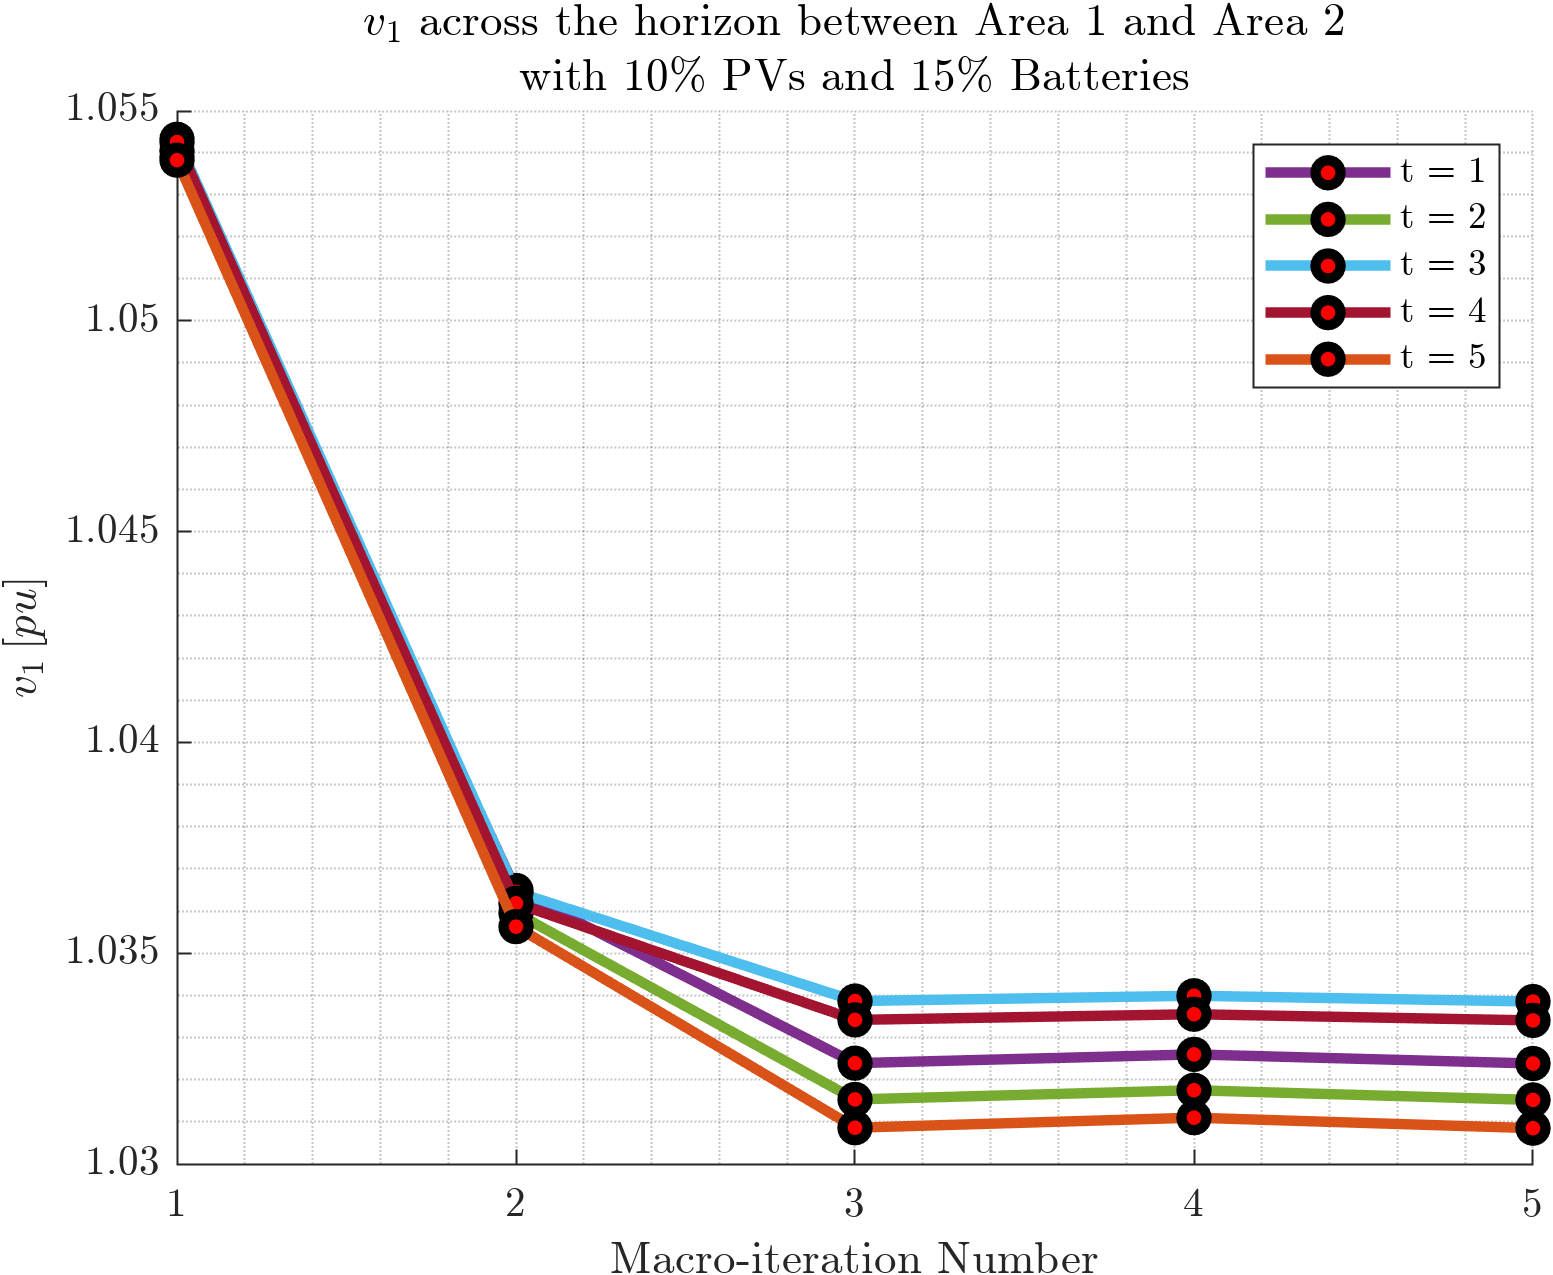
\includegraphics[width=\textwidth]{../figures/T5-pv10-batt15-vBoundary/BoundaryVoltage_vs_t_vs_macroItr_5Areas_1_2_genCost_pv_10_batt_15_.png}
        \caption{Voltage: Area 1 to Area 2}
        \label{fig:voltage_1_2}
    \end{subfigure}
    \hfill
    \begin{subfigure}[b]{0.3\textwidth}
        \centering
        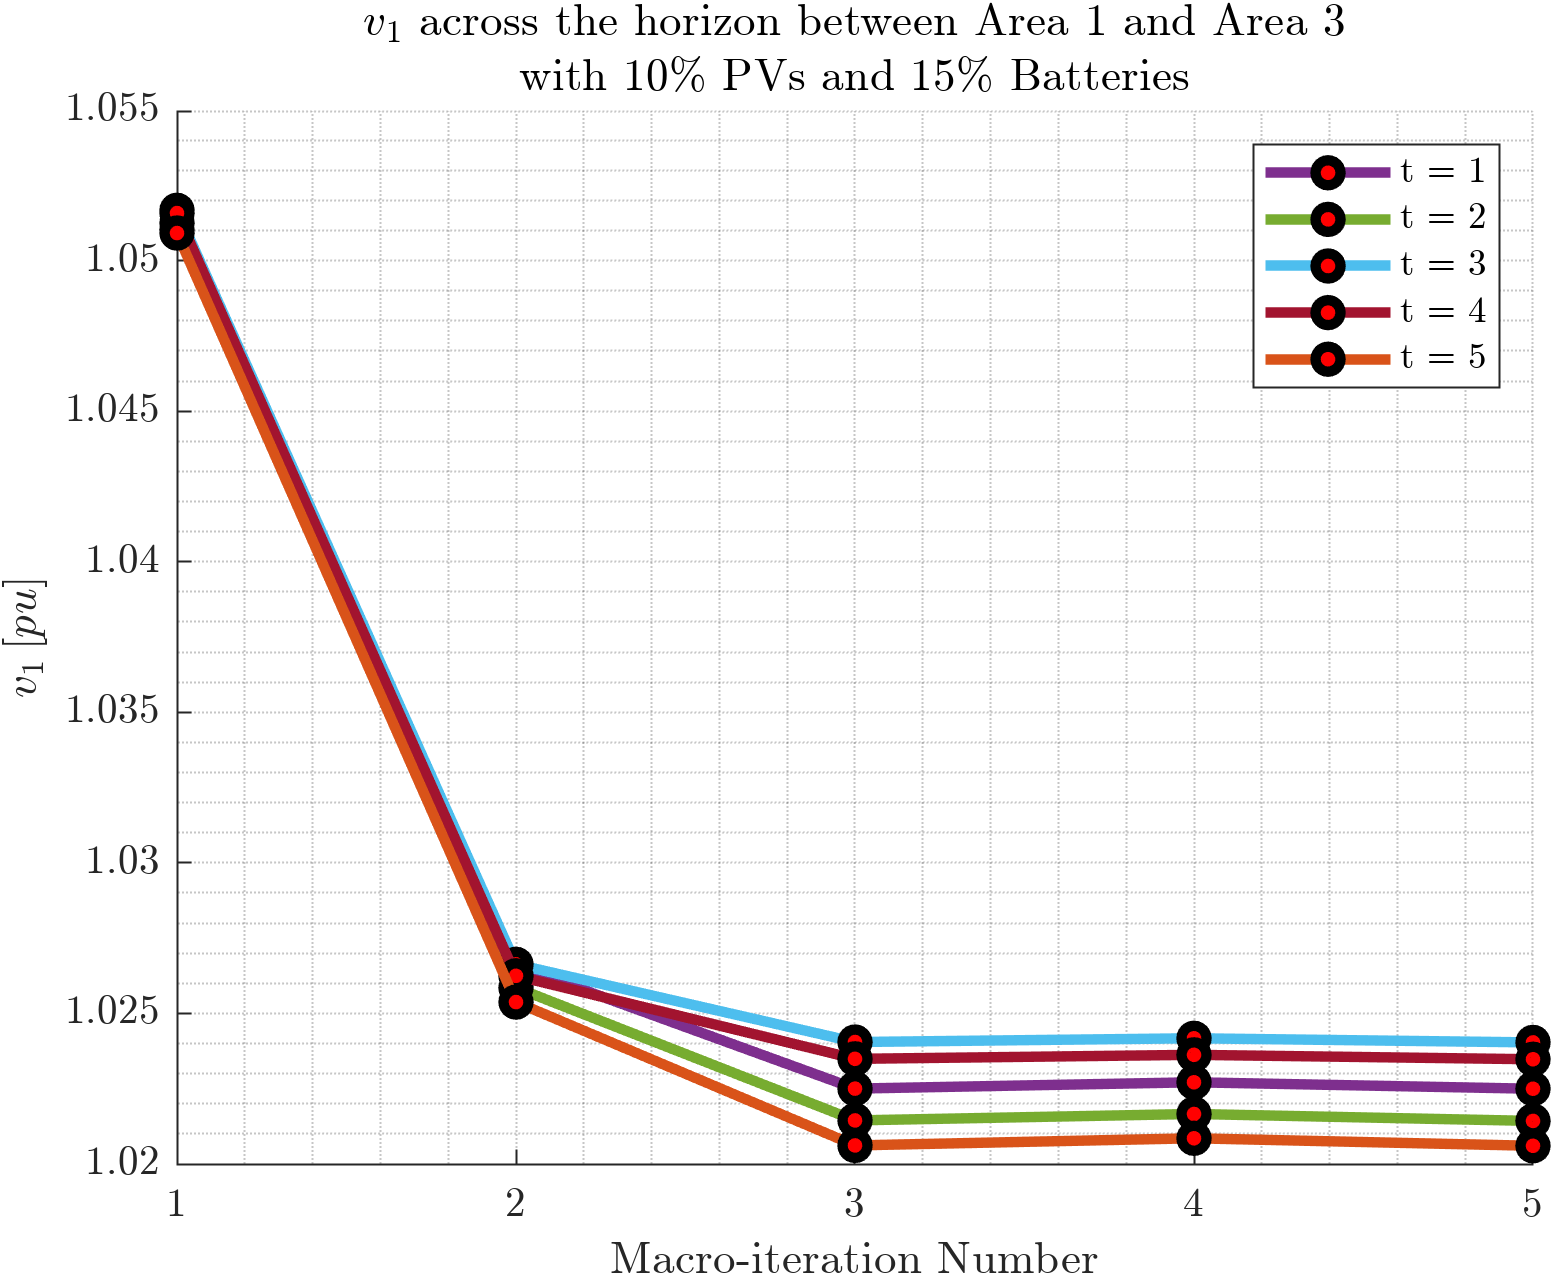
\includegraphics[width=\textwidth]{../figures/T5-pv10-batt15-vBoundary/BoundaryVoltage_vs_t_vs_macroItr_5Areas_1_3_genCost_pv_10_batt_15_.png}
        \caption{Voltage: Area 1 to Area 3}
        \label{fig:voltage_1_3}
    \end{subfigure}
    \hfill
    \begin{subfigure}[b]{0.3\textwidth}
        \centering
        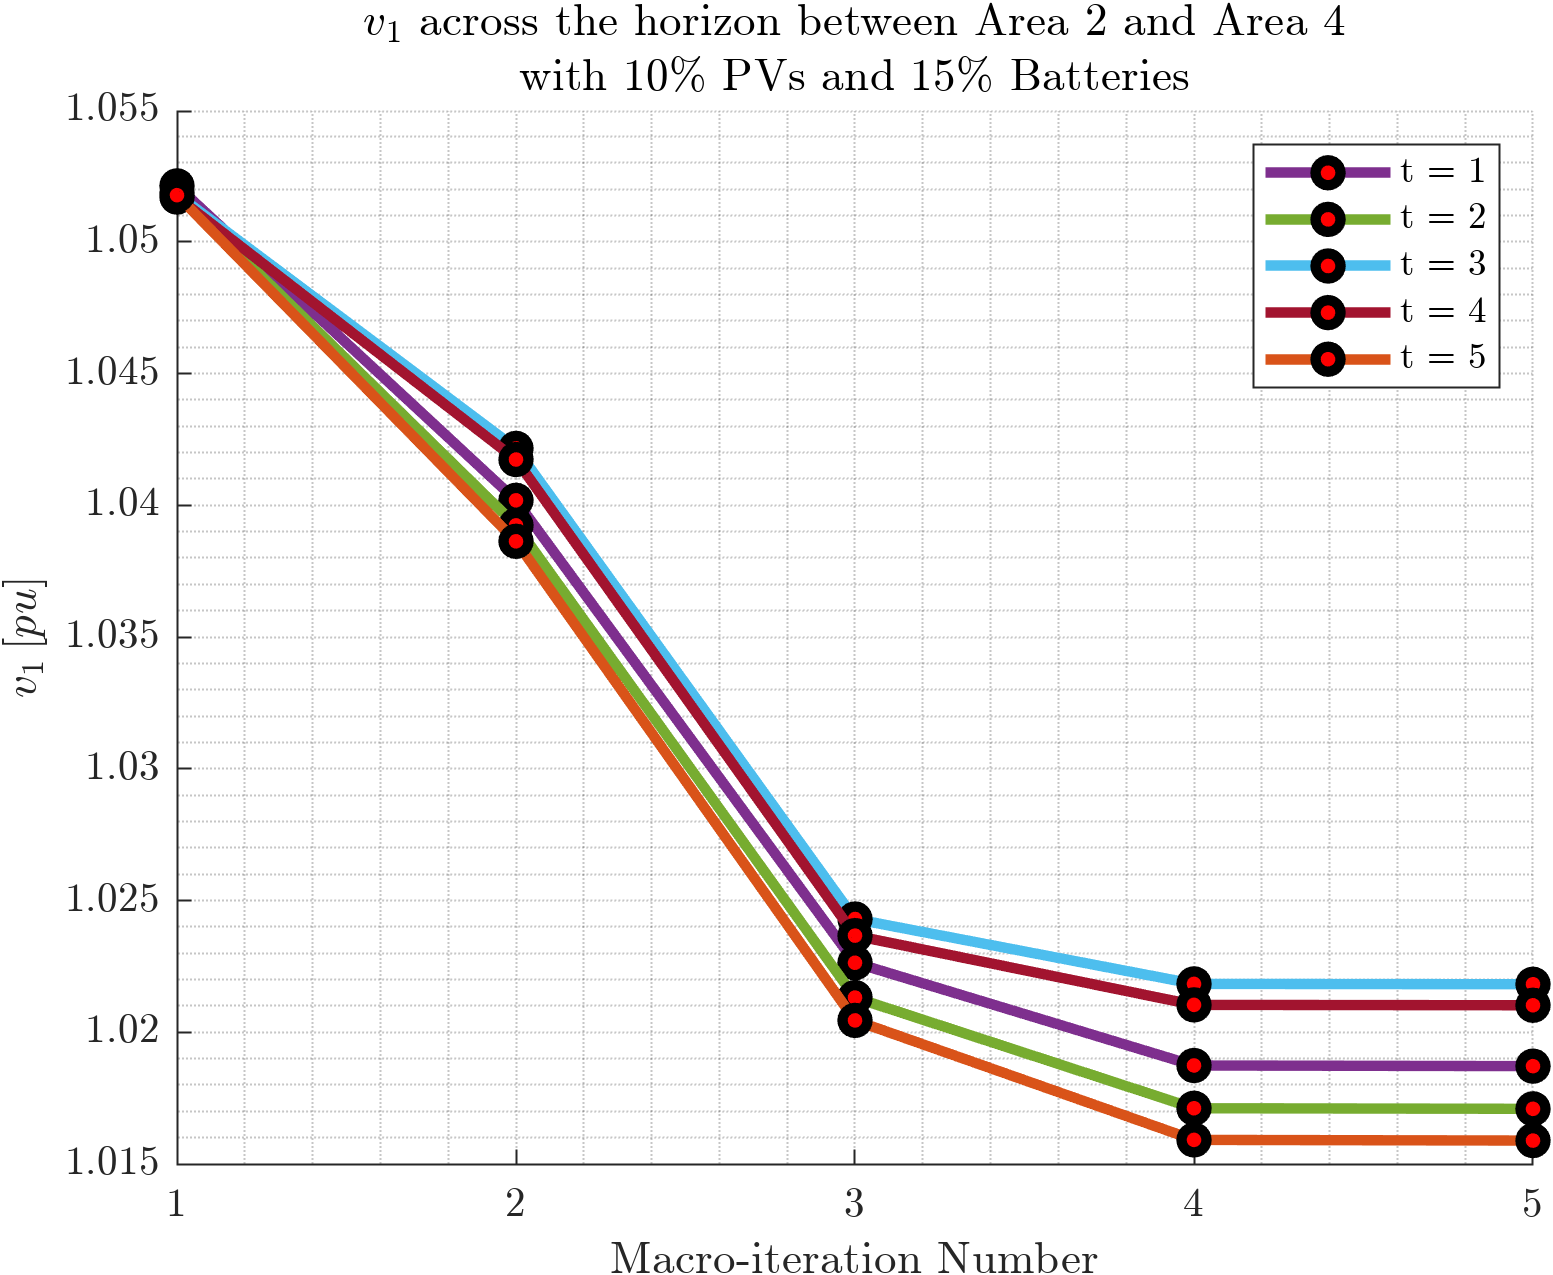
\includegraphics[width=\textwidth]{../figures/T5-pv10-batt15-vBoundary/BoundaryVoltage_vs_t_vs_macroItr_5Areas_2_4_genCost_pv_10_batt_15_.png}
        \caption{Voltage: Area 2 to Area 4}
        \label{fig:voltage_2_4}
    \end{subfigure}

    \caption{Boundary variables exchanged between pairs of areas during each iteration}
    \label{fig:boundary_variables_all}
\end{figure*}


% \begin{figure}[h!]
%     \centering
%     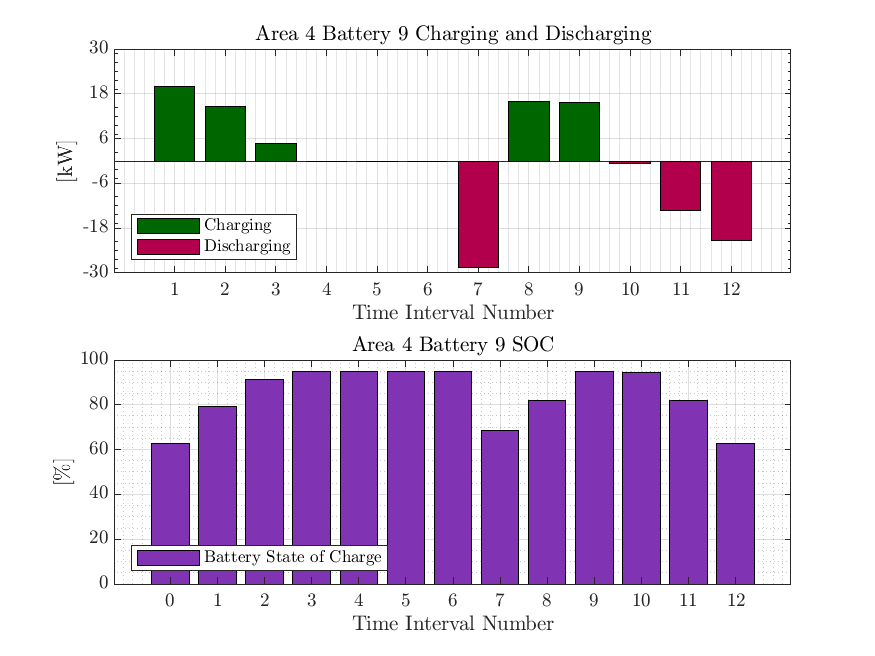
\includegraphics[width=\linewidth]{../figures/T12-pv10-batt15-genCost-peakShave/macroItr_5_genCost_peakShave_Battery_9_alpha_0.001.png}
%     \caption{Charging-Discharging and SOC graphs for Battery 9 located in Area 4}
%     \label{fig:battery_charging_discharging}
% \end{figure}



\subsubsection{Scalability Analysis}

\subsubsection{Comparison between MPCOPF and MPDOPF}
In this section, comparative analyses are carried out between MPCOPF and MPDOPF considering 10-hour time steps with $20\%$ PV penetration and $30\%$ battery penetration.


% \begin{table}[h!]
%     \centering
%     \caption{Comparative analyses between MPCOPF and MPDOPF}
%     \begin{tabular}{|l|c|c|}
%     \hline
%     \textbf{Metric} & \textbf{MPCOPF} & \textbf{MPDOPF} \\ \hline
%     Line loss (kW) &   &  \\ \hline
%     Substation real power (kW) &    &   \\ \hline
%     Substation reactive power (kVAR) &    &   \\ \hline
%     PV real power (kW) &    &    \\ \hline
%     PV reactive power (kVAR) &    &   \\ \hline
%     Substation power cost (\$) &     &   \\ \hline
%     \end{tabular}
%     \label{table:opt-10-20-30}
% \end{table}

\textcolor{red}{Do you want PV Real Power in the table too? (Not controllable, so nothing to compare)}

\begin{table}[h!]
    \centering
    \caption{Comparative analyses between MPCOPF and MPDOPF}
    \begin{tabular}{|l|c|c|}
    \hline
    \textbf{Metric} & \textbf{MPCOPF} & \textbf{MPDOPF} \\ \hline
    Line loss (kW) & 148.67 &  \\ \hline
    Substation real power (kW) & 8544.28 &   \\ \hline
    Substation reactive power (kVAR) & 1092.39 &   \\ \hline
    % PV real power (kW) & 561.26 &    \\ \hline
    PV reactive power (kVAR) & 222.59 &   \\ \hline
    Substation power cost (\$) & 1197.87 &   \\ \hline
    Number of Iterations & 5 &   \\ \hline
    Total Simulation Time (s) (\$) & 4620.73 &   \\ \hline
    \end{tabular}
    \label{table:opt-10-20-30}
\end{table}


Further, here the 

\begin{table}[h!]
    \centering
    \caption{ACOPF feasibility analyses}
    \begin{tabular}{|l|c|c|c|}
    \hline
    \textbf{Metric} & \textbf{MPDOPF} & \textbf{OpenDSS} \\ \hline
    Line loss (kW) &   &  \\ \hline
    Substation real power (kW) &    &   \\ \hline
    Substation reactive power (kVAR) &    &   \\ \hline
    Max. voltage discrepancy (pu) &    &    \\ \hline
    Max. line loss discrepancy (pu) &    &   \\ \hline
    Max. substation power discrepancy (pu) &     &   \\ \hline
    \end{tabular}
    \label{table:feas-copf-10-20-30}
\end{table}

% \begin{table}[h!]
%     \centering
%     \caption{Combined MPDOPF and OpenDSS Results (Substation Power Cost Minimization - 12 Hour Horizon)}
%     \begin{tabular}{|l|c|c|}
%     \hline
%     \textbf{Metric} & \textbf{MPDOPF} & \textbf{OpenDSS} \\ \hline
%     Line Loss & 194.14 kW & 194.05 kW \\ \hline
%     Substation Real Power & 10595.10 kW & 10595.71 kW \\ \hline
%     Substation Reactive Power & 2068.79 kVAr & 2058.30 kVAr \\ \hline
%     PV Real Power & 272.60 kW & 272.60 kW \\ \hline
%     PV Reactive Power & 66.04 kVAr & 66.03 kVAr \\ \hline
%     Battery Real Power & -17.04 kW & -17.04 kW \\ \hline
%     Battery Reactive Power & -83.30 kVAr & -83.30 kVAr \\ \hline
%     Substation Power Cost & \$1424.54 & \$1424.63 \\ \hline
%     Demand Real Power & \multicolumn{2}{c|}{10657.21 kW} \\ \hline
%     Demand Reactive Power & \multicolumn{2}{c|}{5863.79 kVAr} \\ \hline
%     \end{tabular}
%     \label{table:feasibility10-10-15}
% \end{table}

\textcolor{red}{Provide a separate graph for PV, Load forecasts for T = 5 and 10}

% \begin{figure}[h!]
%     \centering
%     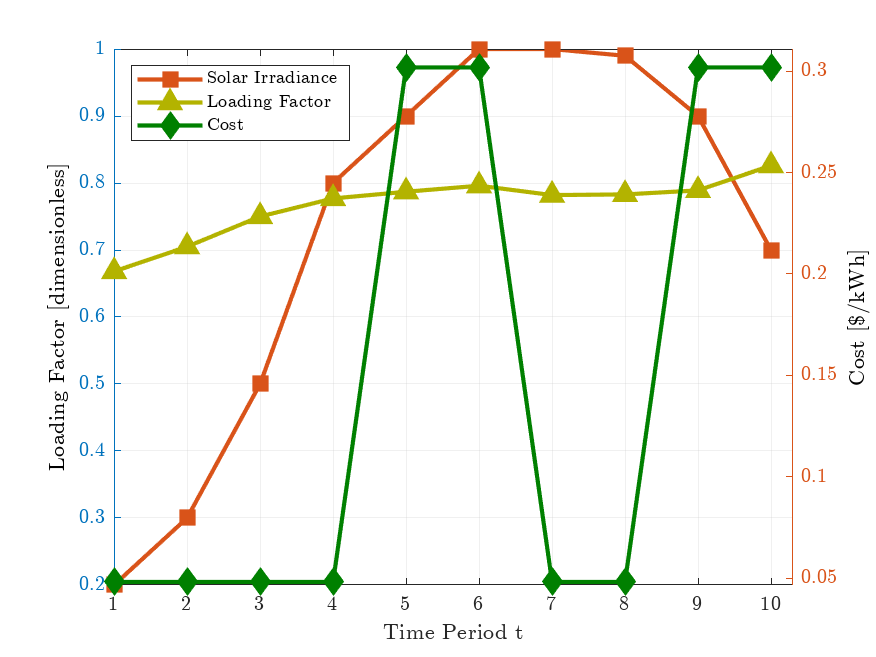
\includegraphics[width=\linewidth]{../figures/T10-inputCurves/InputCurves_Horizon_10_pv_20_batt_30.png}
%     \caption{Time-series comparison for forecasts for Demand Power, Irradiance and Cost of Substation Power over a 10 Hour Horizon}
%     \label{fig:inputCurve-10}
% \end{figure}

\begin{figure}[h!]
    \centering
    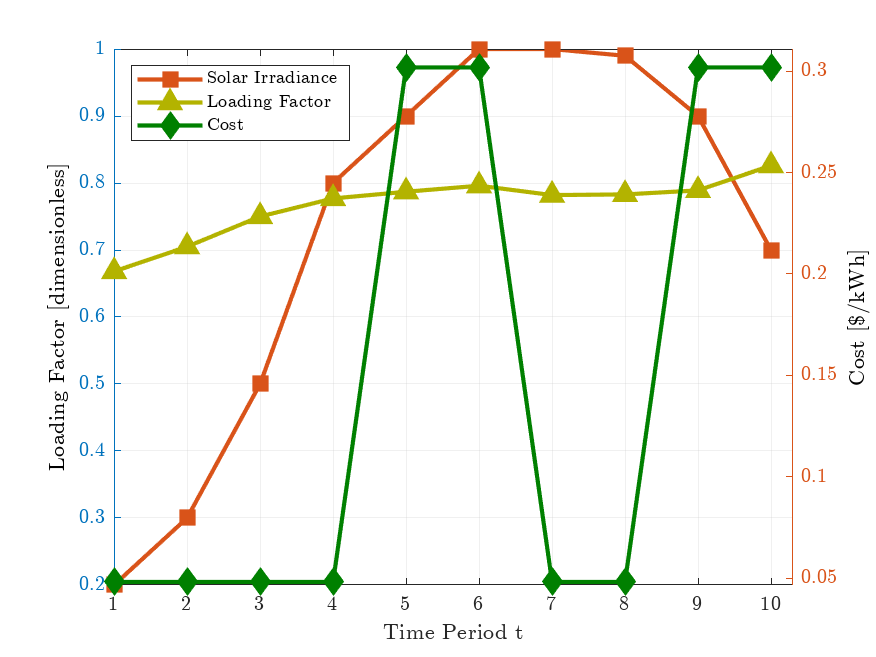
\includegraphics[height=0.25\textheight]{../figures/T10-inputCurves/InputCurves_Horizon_10_pv_20_batt_30.png}
    \caption{Time-series comparison for forecasts for Demand Power, Irradiance and Cost of Substation Power over a 10 Hour Horizon}
    \label{fig:inputCurve-10}
\end{figure}



\begin{figure}[h!]
    \centering
    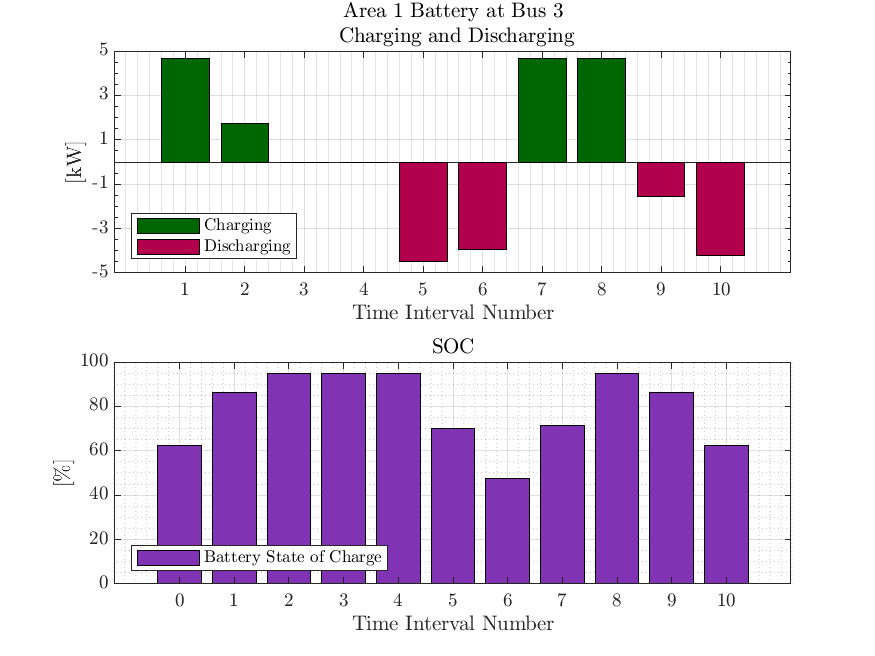
\includegraphics[width=\linewidth]{../figures/T10-pv20-batt30-genCost/copf/BatteryPlots/macroItr_1_genCost_Battery_1_alpha_0.001.png}
    \caption{Charging-Discharging and SOC graphs for Battery at Bus 3 located in Area 1 obtained via MultiPeriodENApp}
    \label{fig:batt-plot-copf-10-20-30-genCost}
\end{figure}
    

\lipsum[1]

\end{document}
